\chapter{Testes e avaliação}

Foi determinada fundamentalmente a necessidade de avaliação do sistema sob duas frentes principais: consumo energético e precisão da posição obtida.

Para tanto, foi elaborado teste para a determinação da precisão na medida da distância entre o ponto de acesso e o \emph{target}. Dada a constante de propagação determinada como 2,95 (ver apêndice 2), foram comparados os valores exibidos pelo ponto de acesso e os medidos por uma trena, os quais estão disponíveis na tabela a seguir.

\begin{table}[ht]
\centering
\caption{Distâncias medidas pelo ponto de acesso e pela trena}
\vspace{0.5cm}
\begin{tabular}{l|cccccccc}
\hline
\makecell{Distâncias pela \\ trena (m)} & 0,5 & 1,0 & 2,0 & 3,0 & 4,0 & 5,0 & 6,0 & 7,0 \vspace{0.4cm}\\

\makecell{Distâncias \\ pelo AP (m)} &
\makecell{0,79 \\ 0,86 \\ 0,73 \\ 0,86 \\ 0,63 \\ 0,63 \\ 0,63 \\ 0,63 \\ 0,63 \\ 0,63 \\ 0,63} &
\makecell{1,00 \\ 1,08 \\ 1,08 \\ 1,00 \\ 1,00 \\ 1,00 \\ 1,08 \\ 0,68 \\ 1,26 \\ 1,00 \\ 1,00} &
\makecell{0,73 \\ 0,73 \\ 0,73 \\ 0,86 \\ 1,37 \\ 1,87 \\ 1,60 \\ 1,50 \\ 1,48 \\ 1,37 \\ 1,48} &
\makecell{8,22 \\ 2,76 \\ 3,22 \\ 2,55 \\ 2,18 \\ 2,18 \\ 2,18 \\ 2,02 \\ 2,18 \\ 2,55 \\ 1,60} &
\makecell{2,15 \\ 1,82 \\ 2,78 \\ 2,56 \\ 2,78 \\ 2,35 \\ 2,56 \\ 3,30 \\ 3,03 \\ 2,78 \\ 2,56} &
\makecell{3,59 \\ 2,56 \\ 4,26 \\ 3,03 \\ 3,91 \\ 8,43 \\ 7,74 \\ 5,05 \\ 6,53 \\ 5,05 \\ 6,53} &
\makecell{4,64 \\ 4,64 \\ 4,64 \\ 3,91 \\ 3,03 \\ 2,56 \\ 2,56 \\ 5,99 \\ 4,26 \\ 14,07 \\ 7,11} &
\makecell{7,04 \\ 5,15 \\ 6,51 \\ 10,40 \\ 7,61 \\ 13,14 \\ 8,90 \\ 3,77 \\ 4,08 \\ 2,98 \\ 4,76}
\vspace{0.4cm}\\

\makecell{Distância média \\ pelo AP (m)} & 0,69 & 1,02 & 1,24 & 2,88 & 2,61 & 5,15 & 5,22 & 6,76
\end{tabular}
\vspace{0.4cm}\\
\centerline{\small{Fonte: autores}}
\end{table}

\begin{table}[ht]
\centering
\caption{Erro quadrático médio e máximo para cada n}
\vspace{0.5cm}
\begin{tabular}{l|c}
\hline
Erro quadrático médio (m) & 1,52 \vspace{0.4cm}\\
Erro quadrático máximo (m) & 3,04
\end{tabular}
\vspace{0.4cm}\\
\centerline{\small{Fonte: autores}}
\end{table}

Dessa forma, foi possível determinar o erro quadrático obtido, que é aproximadamente 1,5m, como pode ser visto na tabela 3, que é um valor aceitável considerando a escala da área local de implementação. Entretanto, ainda é um erro alto para ambientes de cativeiro, cuja área é menor.

\begin{figure}[ht]
  \centering
    \caption{Gráfico das distâncias medidas}
    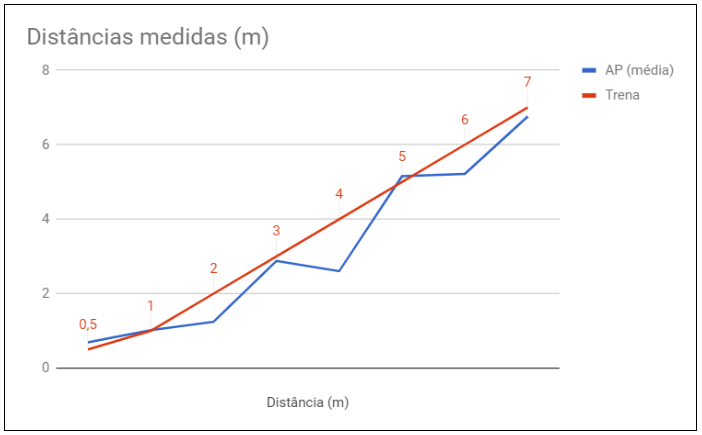
\includegraphics[scale=0.79]{graph-test-dist}
  \centerline{\small{Fonte: autores}}
\end{figure}

\begin{figure}[ht]
  \centering
    \caption{Gráfico do erro quadrático para as distâncias medidas em n=2.95}
    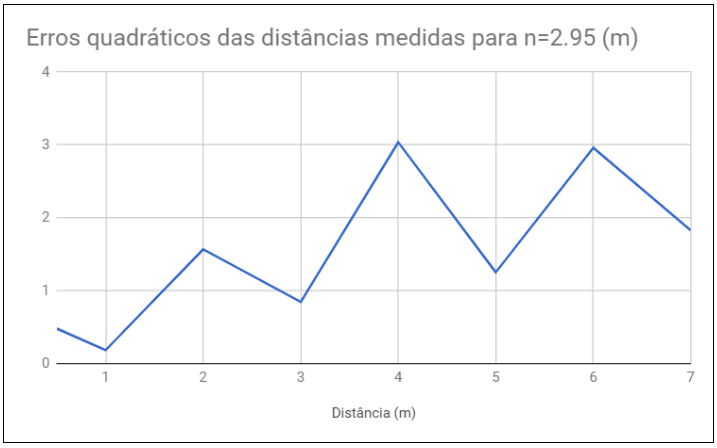
\includegraphics[scale=0.79]{graph-test-erro}
   \centerline{\small{Fonte: autores}}
\end{figure}

No que se refere ao consumo energético, o único teste prático que foi pensado exigiria expor uma bateria nova à exaustão e calcular o tempo tomado. No entanto, como dimensionamos o sistema para que possa durar semanas, este teste é pouco praticável e fica dentro do escopo secundário do projeto.
